\chapter{Implementación}

\section{Software}

Para diseñar una interfaz de usuario real, con la que establecer la base para posteriormente representarla mediante HTML y CSS, se utilizan diversos programas de diseño web.

\begin{itemize}

\item \textbf{Sketch}: Sketch es una aplicación de diseño vectorial, que permite diseñar interfaces para aplicaciones móviles o web de una manera sencilla y con una gran potencia.
\item \textbf{Illustrator}: Esta herramienta de ADOBE , permite el diseño de logotipos de forma vectorial,
\item \textbf{Spectrum}: Programa sencillo que permite crear paletas de colores, de forma que se puedan seleccionar colores complementarios o de gama monocromática y utilizarlos para la interfaz de la aplicación.

\end{itemize}

\section{Tecnologías}

Para la realización de la aplicación web, se ha llevado a cabo un análisis de las tecnologías disponibles y se han seleccionado las que mejor se adaptaban a las necesidades del proyecto.

\subsection{Front-End(Cliente)}

Las dos principales e indispensables tecnologías que se usan para la parte del cliente son: el lenguaje de etiquetas HTML5 y las hojas de etilos CSS3. Estas son dos de las tecnologías fundamentales en las que se basa el desarrollo web.

 \vspace{5 mm}

Con la finalidad de conseguir una apariencia cuidada e intuitiva del sitio web, sin la necesidad de crear las hojas de estilos propias, se consideró la idea de usar el framework Bootstrap. Sin embargo, debido al objetivo de personalizar al máximo la apariencia de la web y a que Bootstrat no permitía muchos grados de libertad en ello, se descartó este framework y se optó por añadir clases propias mediante css.

\vspace{5 mm}

Para maquetar el sitio web con CSS3 de forma más rápida y refactorizable se utiliza \textbf{Sass}. Sass es un lenguaje de preprocesado de CSS, que permite
escribir CSS de forma más cómoda, posibilitando declarar variables,mixins, herencia de clases, etc \cite{sass-doc}. Hay diversas formas de utilizar Sass
en un proyecto. Mediante un programa como Prepros, mediante un automatizador de tareas como Grunt, o mediante un terminal con los comandos de Sass.
Para el proyecto se ha optado usar el terminal para ejecutarlo, ya que es mucho más ligera y consume menos RAM que con programas como Prepros.
Para que empezar a usar Sass en el proyecto, dentro de nuestra carpeta ``padre'' donde se encuentre el CSS, se crea una carpeta Sass donde se incluirán
todos los ficheros .scss. Con el terminal situado en la carpeta padre se escribe sass --watch sass(nombre de la carpeta donde se encuentran los ficheros
.scss). Finalmente, al compilarlo, se generará un fichero style.css que será la hoja de estilo a usar.

\vspace{5 mm}

Para añadir el dinamismo a la web, se ha optado por utilizar un framework de Javascript como \textbf{JQuery} que permite simplificar la manera de
interactuar con los elementos HTML mediante funciones propias. También permite funciones propias para animaciones y peticiones HTTP. Además, JQuery
es software libre \cite{jquery-doc}.

\vspace{5 mm}

Como última tecnología Front-End se utiliza la API de Google Maps, indispensable para el sitio web ya que la principal proposición de valor de la
aplicación es la geolocalización de recetas, y para su representación necesitamos la API de Google.


\subsection{Back-End(Servidor)}

Después de barajar diversos lenguajes para desarrollar el back-end de la aplicación, finalmente se eligió PHP. Además de ser el lenguaje más utlizado
para el desarrollo web, es uno de los lenguajes más potentes y flexibles, pudiendo ser utilizado en la mayoría de los servidores web y sistemas operativos.
Además PHP esta publicado bajo licencia de software libre, por lo que no supone ningun coste.


\vspace{5 mm}

Para montar la arquitectura MVC en la aplicación, se utiliza el framwework Laravel \cite{laravel-doc}. Laravel agiliza el desarrollo de las aplicaciones
web, permitiendo multitud de funcionalidades. Con este framework, desarrollado de forma elegante y simple se evita la creación de código espagueti,
facilitando su refactorización y/o su modificación. Algunas de las características de Laravel:


\begin{itemize}

\item \textbf{Plantillas}. Laravel utiliza platillas Blade. Blade permite tener un sitema de vistas modular de forma que se tenga que repetir la menor
cantidad de código. Para ello se genera una plantilla base o layout, que es donde se representa la estructura de la web y se volcará el contenido para
cada página. Mediante la directiva include(nombre\_template), se podrá incluir una vista parcial de contenido HTML, esta directiva se utiliza para
contenido que no cambia, por ejemplo para incluir la cabecera o el footer de la aplicación. Luego mediante la sentencia yield(nombre\_template),
permitiremos crear una futura sección en el HTML que se definirá en las vistas que son heredadas de este template. Mediante la sentencia
extends(nombre\_template) le diremos a Laravel que vistas se van a usar como futuras secciones. Con estas sentencias se conseguirá volcar el
contenido especifíco para cada página de la web duplicando el menor número de codigo HTML y de forma más modular.

\item \textbf{ORM}. Es una implementación de registro activo para trabajar con la base de datos de forma que cada tabla de la base de datos tiene un
Modelo correspondiente asociado con el mismo nombre. Esta implementación permite también métodos predefinidos para llamar a la base de datos como:
save(),create(),get(),find() \cite{eloquent-orm}.

\item \textbf{Caché}. Laravel, cuenta con un robusto sistema de caché, el cual se puede ajustar, para que se produzca una carga rápida de la web y
generar una mejor experiencia al usuario.

\item \textbf{MiddleWare}. Usa HTTP Middleware, que proporcionan un correcto mecanismo para filtrar las peticiones en la aplicación. Un ejemplo de
middleware que incluye Laravel, es el usado para verificar si el usuario esta autenticado en la aplicación.

\end{itemize}

\vspace{5 mm}

Para la base de datos, se utiliza el sistema de gestión relacional MySQL, ya que es uno de los sistemas más utilizados y con mayor documentación para el
desarrollo web. Además, de la perfecta integración con Laravel.

\subsection{Estructura de la aplicación}

Para comenzar a desarrollar el proyecto, primero se debe instalar Laravel. Para ello se utiliza un manejador de dependencias como composer que nos
permite instalar los paquetes y librerías de forma automática sin la necesidad de hacerlo de forma manual. Mediante nuestro terminal escribimos el
siguiente código para instalar composer en el ordenador: curl -sS https://getcomposer.org/installer | php. Una vez instalado, para
generar un proyecto con Laravel escribimos en el terminal el siguiente comando: composer create-project laravel/laravel nombre-proyecto.

\vspace{5 mm}

Si vamos a la carpeta raíz con la que creamos el proyecto se observa que dentro composer ha generado una estructura de directorios que es como organiza
Laravel el código de la aplicación. A continuación se detallan brevemente cada una de ellas:

\begin{itemize}

\item \textbf{app}. El directorio app es donde se encontrará la mayor parte del código personal del back-end de la aplicación. Desde los modelos de datos de la aplicación, hasta los controladores pasando por el middleware.

\item \textbf{config}. Aquí se encuentran los ficheros de configuración de Laravel y de la aplicación. Por ejemplo en el fichero app.php se especifican parametros tales como la zona horaria y el idioma de la aplicación. También se definen los providers, que son cada uno de los objetos o instancias que se cargarán en el proyecto.

\item \textbf{database}. Aquí se encuentran todos los ficheros relacionados con la base de datos de la aplicación. Dentro encontramos tres subdirectorios:

- factories: aquí se incluyen los ficheros que generan automaticamente nuevos datos en tu base de datos para testear la aplicación, sin necesidad de generarlos manualmente.

- migrations: las migraciones son un tipo de control de versiones para la base de datos. A través de estos ficheros se puede modificar la base de datos.

- seeds: permiten poblar la base de datos con datos de prueba. Los seeds pueden utilizar factories para poblar la base de datos o introudcirlos manualmente.

\item \textbf{public}. En este directorio se encuentran los directorios con ficheros estáticos como son las hojas de estilo(css), los ficheros javascript(js) y las imágenes(images).

\item \textbf{resources}. En resource encontramos subdirectorios donde se encuentran las vistas  en formato blade.php de la aplicación(views) y los archivos de idiomas de la aplicación, para poder pasar de un idioma a otro en la aplicación(lang).

\item \textbf{storage}. Se encuentran varios subdirectorios que contiene el cache de la aplicación, sesiones, etc.

\item \textbf{vendor}. Este directorio contiene todo el core de Laravel y los componentes instalados.

\end{itemize}


\textbf{Estructura Sass}

Como se comenta previamente, se utiliza Sass para maquetar la web. Este lenguaje de preprocesado de CSS permite organizarlo y hacerlo más modular de
forma que se pueden generar varios ficheros .scss y compilarlos en un único fichero CSS que es el que se utilizará en la aplicación. Para ello se usa
una carpeta sass que se incluye en la carpeta public del proyecto donde se incluyen todos los directorios con los ficheros .scss. Una de las formas de
refactorizar más el código Sass, es generar un fichero .scss para cada página web de la aplicación de modo que en futuros cambios resulte todavía más
sencillo modificar el estilo. La estructura Sass es al siguiente:


\begin{itemize}

\item \textbf{base}: en el directorio base se encuentran los ficheros scss con los elementos más básicos de la aplicación. Las tipografías usadas, los formatos de texto de los encabezados y párrafos, etc.

\item \textbf{config}: en este directorio encontramos los siguientes ficheros.

- variables: scss donde se declaran las variables que se usan en las hojas de estilo tales como colores de la aplicación, las fuentes usadas.

- functions: aquí se encuentran los mixins de sass que se pueden utilizar. Los mixins no son más que funciones que permiten reutilizar estilos.

- animations: en este directorio se incluyen los ficheros scss con animaciones hechas con css incluidas en la aplicación.

\item \textbf{ui}: en el directorio ui(user interface) se incluyen los ficheros scss que modifiquen las propiedades css de elementos de la interfaz gráfica de la aplicación como botones,formularios, etc.

\item \textbf{modules}: debido a que la aplicación esta basada en la filosofía mobile first en esta carpeta se incluyen todos lo ficheros scss de las páginas de la aplicación en resolución móvil(de 0 a 768px de resolución de pantalla).

\item \textbf{mediaqueries}: en esta carpeta se incluyen los ficheros scss para las resoluciones de tablet y ordenador de escritorio. Para esta resolución se han marcado las resolución de 768px a 1024px(tablet) y para escritorio las resoluciones de 1024px a 1600px y mayores de 1600px. Para cada resolución habrá un subdirectorio con el nombre de la resolución donde se incluirán sus ficheros scss correspondientes.


\end{itemize}

\vspace{5 mm}

\section{Sprints}

Una instalado el framework Laravel y comprendida su estructura se procede a desarrollar la aplicación. Para realizar el proyecto, como se especifica previamente se utiliza la metodología Scrum. El proyecto se divide en los siguientes sprints:


\subsection{Diseño de la interfaz}

\begin{figure}
\begin{center}
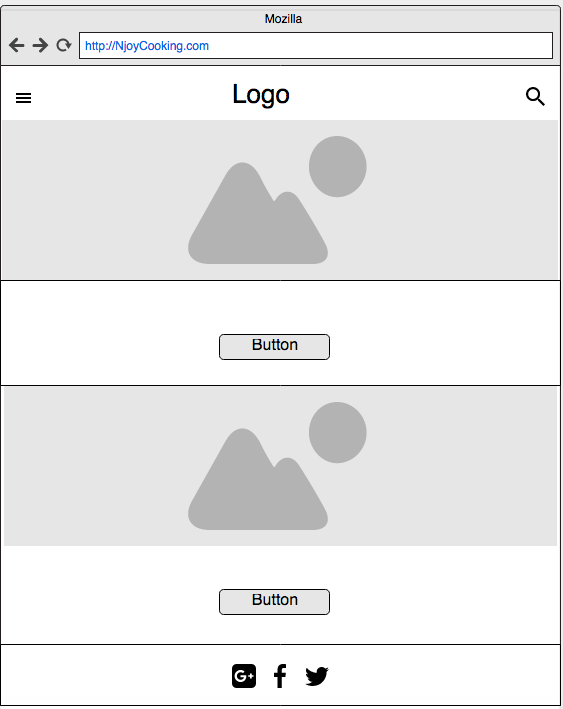
\includegraphics[width=1.0\textwidth]{imagenes/landing.png}
\caption{Landing}
\label{landing}
\end{center}
\end{figure}

\begin{figure}
\begin{center}
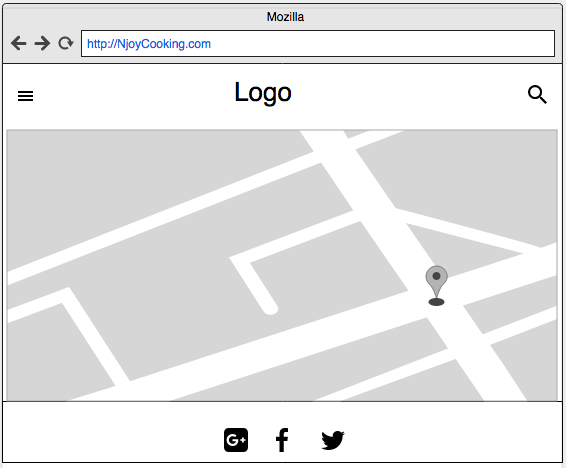
\includegraphics[width=1.0\textwidth]{imagenes/mapa.png}
\caption{Mapa}
\label{mapa}
\end{center}
\end{figure}

\begin{figure}
\begin{center}
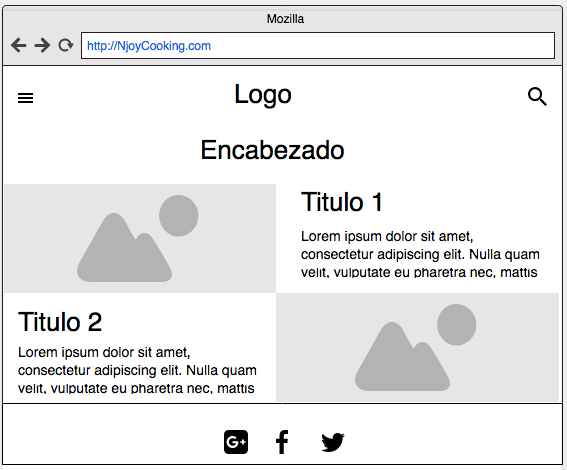
\includegraphics[width=1.0\textwidth]{imagenes/listado-blog.png}
\caption{Listado de noticias}
\label{listado-blog}
\end{center}
\end{figure}

\begin{figure}
\begin{center}
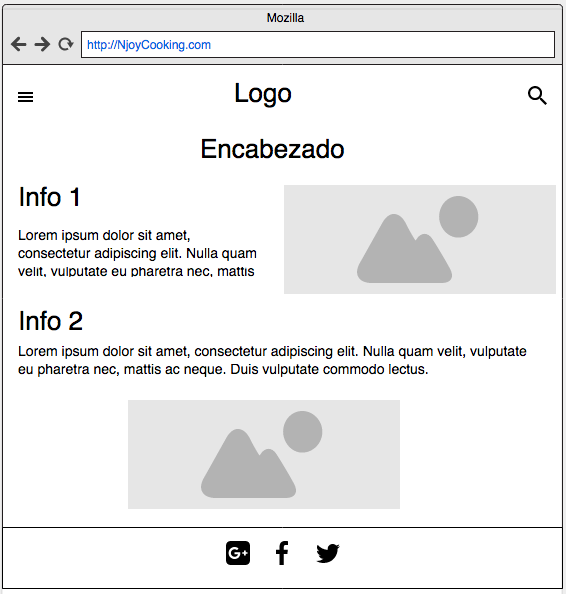
\includegraphics[width=1.0\textwidth]{imagenes/detalle-blog.png}
\caption{Detalle de noticia}
\label{detalle-blog}
\end{center}
\end{figure}

\begin{figure}
\begin{center}
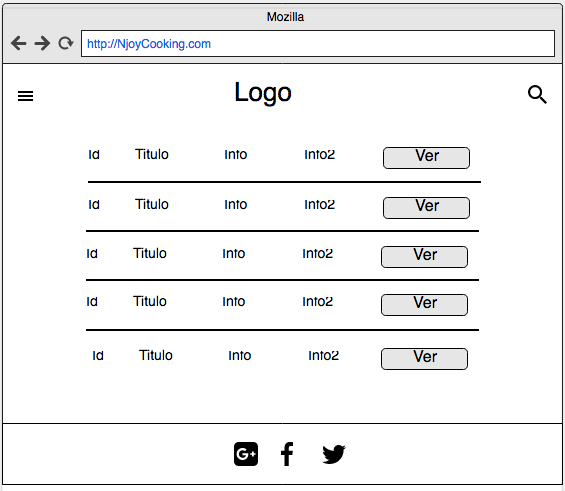
\includegraphics[width=1.0\textwidth]{imagenes/listado-admin.png}
\caption{Listado de elementos}
\label{listado-admin}
\end{center}
\end{figure}

Inicialmente se llevan a cabo unos bocetos de la web mediante mockups para saber como se va a organizar el contenido de la aplicación.

\vspace{5 mm}

Cualquier empresa que se encuentre en el mundo de las aplicaciones web sabe que una landing, es la mejor forma de promocionar el producto o marca que se quiere dara conocer. Por eso a la página inicial donde el usuario accederá será una landing donde se mostrará información acerca de los servicios que ofrece la web.

\vspace{5 mm}

Como se observa en el boceto(figura \ref{landing}) la landing tiene un diseño sencillo y usable. En esta página se mostrarán una series de secciones informativas acerca de los contenidos disponibles de la web y otras informaciones relevantes. Las secciones irán acompañadas de una imagen de fondo, un texto informativo y un botón que dirige a la página correspondiente.

\vspace{5 mm}

La cabecera de la landing, que será común a todas las páginas de la web, tendrá un diseño responsive para todas las resoluciones. El menú será desplegable de forma que al pulsar sobre el icono de  la hamburguesa se verán todas las secciones por las que se podrá navegar por la web. Este menú mobile se ha aplicado para la resolución de escritorio ya que favorecía a conseguir una mayor limpieza de la interfaz,no empeoraba su usabilidad y le daba un aspecto más minimalista. Además de este menú en la cabecera encontraremos el logo de la web y un buscador global de la web. Esta cabecerá siempre estará fija para favorecer la usabilidad al usuario.

\vspace{5 mm}

Por último, el footer o pie de página, otro elemento común a todas las páginas. En esta sección se mostrarán las distintas redes sociales de la empresa, los textos legales(copyright,privacidad) y el logo de la web.


\vspace{5 mm}

La siguiente página, es la del mapa (figura \ref{mapa}). En esta página se mostraban un mapa con los marcadores de las recetas geoposiconadas. El diseño de esta página es muy sencillo ya que además de los elementos comunes de cabecera y pie, en el contenido se muestra un elemento con el mapa que va a mostrar la información.

\vspace{5 mm}

La próxima sección, es la sección del blog que se compone de dos páginas: el listado de noticias y el detalle de noticia. En el listado de noticias(figura \ref{listado-blog}), el primer elemento que se mostrará será un encabezado con una foto y descripción de la sección del blog. A continuación se mostrarán un listado con las diferentes noticias del blog y en cada una se mostrará un foto, un título y un resumen. Para esta sección la disposición de los elementos de la notícia en movil cambiará colocando los elementos en una sola columna en vez de dos como se muestran en tablet y pc.

\vspace{5 mm}

En el detalle de la receta(figura \ref{detalle-blog}) se muestra toda la información asociada a esa noticia. El primer elemento que aparece es el encabezado de la noticia donde se muestra su título y una foto de fondo. A continuación se muestra en dos columnas la información de la receta, una columna con un primer bloque de información y la segunda con la imagen principal de la noticia. Después se muestran los demás bloques de información en una sola columna y por último se muestran otra fotos asociadas a la noticia. Al final de la noticia se muestra un formulario para escribir comentarios asociados a la noticia y un listado con los comentarios que tiene la noticia. La estructura del contenido cambia para la resolución móvil mostrando todo el contenido en una columna.

\vspace{5 mm}

Si el usuario que accede a la página esta registrado, aparecerán nuevas secciones disponibles. Estas secciones serán vistas como listados de elementos(figura \ref{listado-admin}), se usaran para mostrar cualquier tipo de datos que visualice el usuario registrado. La información se listará en una disposición de tabla, con el contenido del elemento(id,titulo,etc) y un botón para ver el detalle. La presentación de este contenido es mucho más simple, que el listado para los usuarios no registrados, ya que esta sección tiene que ser mucho más pragmática y menos visual.

\vspace{5 mm}

\textbf{Paleta de Colores}

\vspace{5 mm}

\begin{figure}
\begin{center}
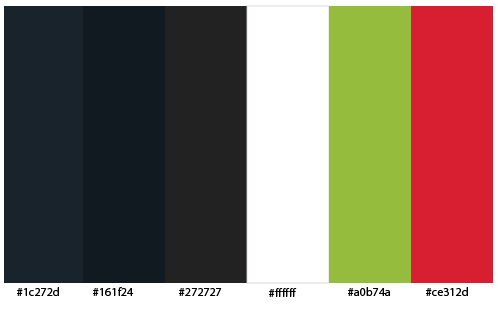
\includegraphics[width=1.0\textwidth]{imagenes/paleta.png}
\caption{Paleta de Colores}
\label{paleta}
\end{center}
\end{figure}

Para la aplicación se ha seleccionado una paleta de colores(\ref{paleta}) con el programa spectrum. Se ha elegido una gama de azules y grises oscuros que dan un aspecto de seriedad y confianza. También se utilizan una series de colores mas vivos como el verde y el rojo que se utilizan para los botones, pequeños detalles y resaltar los textos para dar una aspecto más vivo.


\subsection{Implementación de la arquitectura}

\begin{figure}
\begin{center}
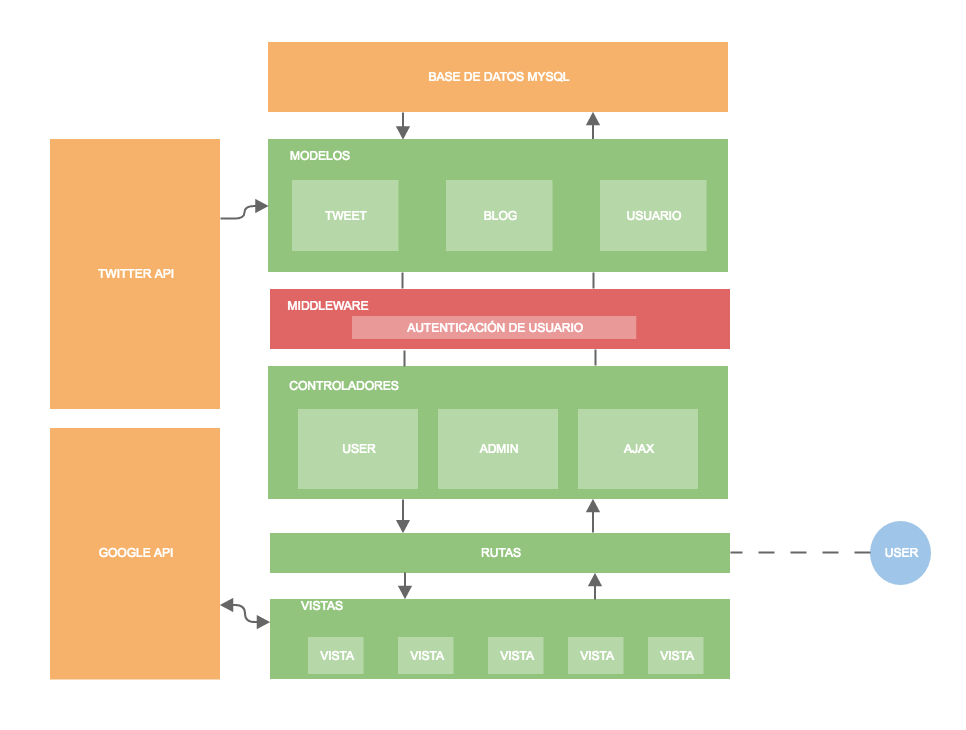
\includegraphics[width=1.0\textwidth]{imagenes/implementacion-arquitectura.png}
\caption{Arquitectura específica}
\label{implement-arch}
\end{center}
\end{figure}

\begin{figure}
\begin{center}
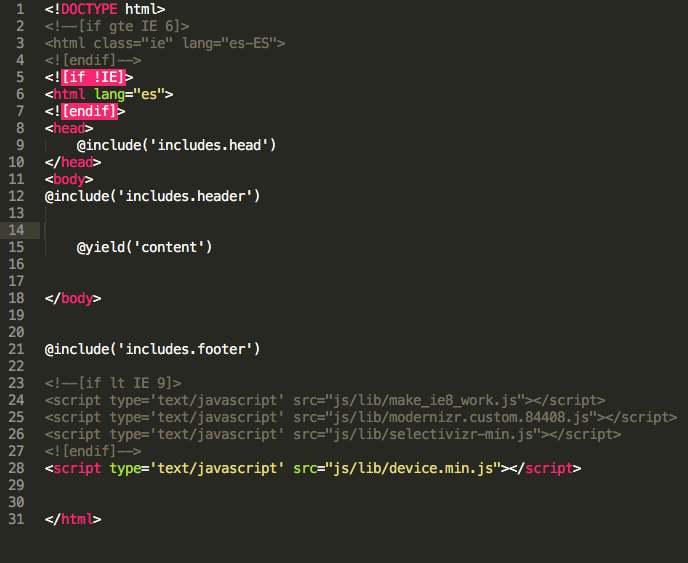
\includegraphics[width=1.0\textwidth]{imagenes/layout.png}
\caption{Layout}
\label{layout}
\end{center}
\end{figure}

En el segundo sprint del proyecto, se lleva acabo un esquema específico de la arquitectura usada para la aplicación. En este esquema de arquitectura ya no es tan general, se especifican detalladamente cada una de las capas de la arquitectura,se enumeran cada uno de los elementos que se va a componer y se detallan cada una de las APIs externas empleadas.

\vspace{5 mm}

En la figura \ref{implement-arch} se observa un esquema detallado de como se ha implementado la arquitectura de la aplicación. A continuación se procede a profundizar en cada una de las capas de la arquitectura.

\vspace{5 mm}

El usuario que navegue por la aplicación, accederá a las diferentes páginas de la web por medio de una ruta que introduzca en el navegador. Una vez introducida la ruta comienza el flujo de información de la aplicación.

\vspace{5 mm}

Con la ruta introducida, la aplicación nos manda al controlador correspondiente para obtener la información. Para organizar mejor la información, se estructuran los siguientes controladores:

\begin{itemize}

\item \textbf{Controller}. Controlador principal de la aplicación, en esta clase se manejan todas las rutas de la aplicación. Este controlador comprueba que la ruta introducida sea correcta, dirigiendo al controlador de cada apartado de la página o por el contrario mostrando la página de error si la ruta es incorrecta.En el constructor de este controlador se crean instancias del resto de controladores en el constructor que luego se llaman para renderizar las distintas vistas de la web.

\item \textbf{AjaxController}. En este controlador se manejarán todos los datos realizados con peticiones ajax. Apartados como los comentarios, utilizarán peticiones ajax para guardar la información en la base de datos y no tener que recargar la página.

\item \textbf{SiteController}. Contiene los métodos que manejan la información correspondiente a la parte pública de la web. El mapa, el blog y la landing se gestionan mediante este controlador.

\item \textbf{AdminController}. La parte privada, es decir aquellas vistas que requieran de autenticación. La gestión de las noticias del blog, los tweets del mapa, se gestionarán con este controlador.

\end{itemize}


En los controladores se hace uso de los diferentes modelos de datos de la aplicación. Los modelos generalmente se corresponden con una tabla de la base de datos. Para cada objeto de datos se crea la clase php(el Modelo) donde se encuentran los métodos que insertan, borran o actualizan la información de su tabla correspondiente.

\vspace{5 mm}

Para obtener los datos de la API twitter, se utiliza la librería TwitterAPIExchange \cite{tweet-framework}, facilitando la obtención de tweets y disponiendo al desarrollador de diversos métodos de búsqueda de resultados. Los datos obtenidos mediante la librería se parsean y se guardan en la base de datos de la aplicación mediante su modelo de datos(Tweet).

\vspace{5 mm}

Una vez obtenida la información en los controladores, se le pasan los datos a la vista que corresponde para visualizar el contenido. Las vistas estan envueltas en un layout, que contiene la estructura de la aplicación y los trozos de la web que son comunes para toda la web, como la cabecera y el pie de página. En el layout de la aplicación (figura \ref{layout}) se observa su estructura. Mediante la sentencia include incrustamos los elementos comunes de la aplicación en el layout(footer y cabecera) y finalmente mediante yield se vuelca el contenido de la vista. Existen varias vistas en la aplicación y cada una tendrá sus estructura HTML y sus características propias.

\vspace{5 mm}


En la parte de cliente, una vez renderizada la vista se hace uso de la API de Google Maps mediante Javascript para generar el mapa de la aplicación y todos sus elementos(marcadores,ventanas de información).

\vspace{5 mm}

Para comprobar la autenticación del cliente, y que cualquier usuario no pueda acceder a partes de la web que solo están disponibles para el administrador, se implementa una capa intermedia entre los controladores y los modelos llamada middleware. Esta capa controla que, el usuario que intenta acceder a las páginas disponibles solo para el administrador, esté registrado como usuario en la base de datos y tenga una sesión iniciada como usuario. Por el contrario si no está registrado, el usuario no podrá acceder y será redirigido a la página principal.

\subsection{Maquetación}

Una vez implementada la arquitectura y definidas las vistas de la aplicación, el siguiente sprint consta de la maquetación de la web.

\vspace{5 mm}

Previamente se estructuran todos los ficheros PHP con contenido HTML en directorios para organizar mejor la aplicación y que las vistas sean más reutilizables:

\begin{itemize}

\item \textbf{layouts}: aquí se incluye la plantilla main con la estructura de la aplicación.

\item \textbf{includes}: en este directorio se incluiran los ficheros que contiene fragmentos parciales de HTML. Estos fragmentos pueden ser tanto elementos fijos de la web como la cabecera o el pie que se incrustan en la estructura principal o render parciales de una vista para estructurar mejor el contenido.

\item \textbf{site}: aquí se incluyen todas las vistas de la aplicación que tienen asociadas un controlador a ellas, como puede ser la página del blog y del mapa.

\item \textbf{error}: en este directorio se incluyen todas las plantillas para mostrar los errores de la web. El error más común es el 404 de la página no encontrada.

\item \textbf{auth}: en la carpeta auth se incluyen los ficheros de autenticación del usuario, como el login del usuario.

\end{itemize}

La estructura HTML de las vistas sigue una jerarquía de las etiquetas que se aplica para generar un contenido más limpio de las vistas y pasar con éxito el validador del W3C garantizando una correcta escritura de HTML.

\vspace{5 mm}


Uso de la etiqueta <section> para dividir las partes de la vista. Cada vista se puede componer de uno o más sections. Por ejemplo para la página de blog se divide con dos sections, una para el bloque de introducción del blog y otra para el listado de noticias. Dentro de cada <section> van las etiquetas que se usarán para posicionar el elemento y darle estilos como son las <div>,<ul>,<span> y <p>.

\vspace{5 mm}

\begin{figure}
\begin{center}
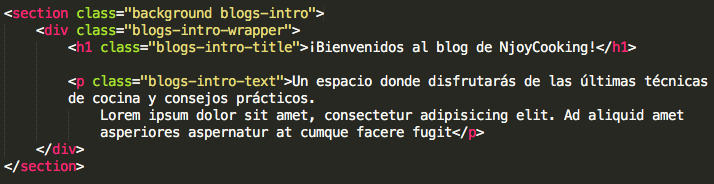
\includegraphics[width=1.0\textwidth]{imagenes/jerarquia-clases.png}
\caption{Ejemplo de jerarquía de clases}
\label{clases-html}
\end{center}
\end{figure}

\begin{figure}
\begin{center}
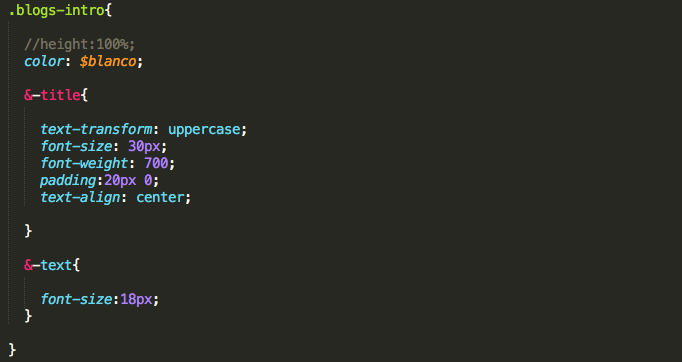
\includegraphics[width=1.0\textwidth]{imagenes/jerarquia-sass.png}
\caption{Ejemplo de jerarquía Sass}
\label{jerarquia-sass}
\end{center}
\end{figure}

Cada etiqueta HTML tiene una clase asociada. Las clases son muy importantes ya que pemiten clasificar los elementos para luego poder aplicarle unas reglas CSS comunes. La nomenclatura que se usa para las clases, es una anidación de palabras clave, seguidas de un guión(-). Por ejemplo para el bloque de la intro del blog(\ref{clases-html}) esta el <section> con la clase que contiene la anidación de palabras blogs-intro. Con esta nomenclatura se hace referencia a que es este elemento pertenece a la vista del blog(blog) y la sección de introducón(intro). Dentro de este elemento, se encuentra una etiqueta <div> que contien los elementos y por eso la nomenclatura de la clase es blogs-intro-wrapper(wrapper es una palabra inglesa que significa envoltura). Por último los dos elementos de la sección son los textos, el blogs-intro-text y blogs-intro-title para estas dos clases se le anida como última palabra text o title para aplicar las reglas a cada tipo de texto dentro del bloque de introducción.

\vspace{5 mm}

Aplicando esta nomenclatura de anidación de palabras clave y gracias a la posibilidades que da Sass, se crea una jerarquía de clases en Sass que permite optimizar al máximo las reglas de estilos de cada elemento evitando tener que duplicar reglas, obteniendo una visión más clara de como está organizado y facilitar modificaciones posteriores por parte de cualquier desarrolador. Un ejemplo de la jerarquía Sass sería la figura \ref{jerarquia-sass}.


\vspace{5 mm}

Para los elementos que son manipulados con jQuery, se les añade un clase extra con el prefijo js-nombre. De forma que cualquier elemento que tenga un evento de jQuery asociado, deberá ser seleccionado mediante la clase con el prefijo js. Estas clases no tendrán estilos asociados, de forma que las clases se dividirán en dos tipos: los selectores de elementos de jQuery y las clases con reglas de estilos asociados. De esta forma estará mejor clasificada la maquetación de los elementos y permitirá que las futuras restructuraciones de la web no supongan tanto trabajo, ya que si únicamente se quiere modificar la apariencia del sitio o optimizar el rendimiento de la web cambiando el código javascript, solo se tendrá que modificar una de los dos tipos de clases sin alterar la otra.


\subsection{Programación}

\begin{figure}
\begin{center}
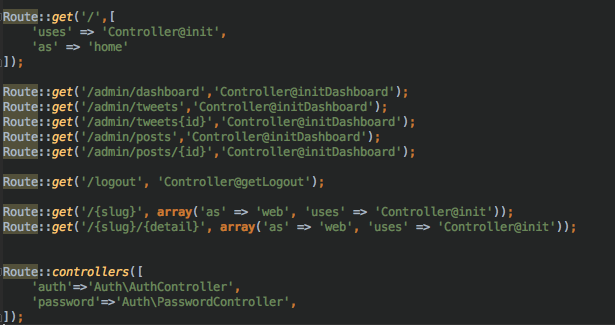
\includegraphics[width=1.0\textwidth]{imagenes/routes.png}
\caption{Rutas de la aplicación}
\label{rutas-app}
\end{center}
\end{figure}


Una vez terminada la maquetación de las páginas, se procede a la programación del back-end de la aplicación. Este apartado es el más extenso de desarrollar por lo que se divide en tres sprints: rutas de la aplicación, lógica de negocio y servicios.

\vspace{5 mm}


\textbf{Rutas de la aplicación}

Para tener una web con un sistema de rutas amigables que faciliten la navegación del usuario y el posicionamiento del sitio, la mejor opción es generar rutas dinámicas. Mediante las rutas dinámicas el administrador del sitio podrá modificar los valores de las rutas mediante el panel de administración, modificando las urls de cada página cuando sea necesario sin la necesidad de recurrir al programador. Otros campos que el administrador también podrá modificar son los metas de cada página(MetaTitle,MetaKeywords,etc), que son otro factor importante para el posicionamiento SEO.

\vspace{5 mm}

Para definir las rutas, Laravel proporciona el fichero routes.php dentro del directorio app que es donde se definen todas las rutas de la aplicación. Dentro de este fichero se definen las rutas especificando el tipo de petición Http(get,post,etc)el nombre de la ruta y el controlador que usa, también podemos definir un alias que identifica la ruta aunque este campo es opcional. Como se observa en la figura \ref{rutas-app} se definen 4 rutas:

\begin{itemize}

\item \textbf{Ruta Principal}: la ruta para la pagina principal donde se mostrará la landing se define mediante el caracter "/". a esta página se accederá cuando el usuario acceda al dominio de la aplicación.

\item \textbf{Rutas de Menu}: estas rutas son las páginas de la aplicación que pertenecen al modelo de datos Menu que se corresponde con el menú de navegación de la web. Se generan dinamicamente comprobando que la ruta obtenida se corresponde con la ruta definida en el modelo. Para que la ruta sea dinamica en Laravel se tiene que definir mediante llaves y dentro un nombre de variable.

\item \textbf{Rutas de detalle}: las rutas de detalle son aquellas que tienen tienen como trozo de url padre una ruta de Menu. No todas las rutas de Menu tienen que tener una ruta de detalle. Esta ruta se usa en la aplicación para definir las noticias del blog de la aplicación y asi poder concatenar a la ruta del blog el nombre de la noticia.

\item \textbf{Rutas de usuario registrado}: estas rutas son para la vistas de la web de la parte de administrador. También son dinámicas pero para diferenciarlas de las rutas visibles para todos los usuarios se iniciarán con la ruta /admin.

\end{itemize}


Todas estas rutas se manejan en el controlador principal de la aplicación(Controller). Se comprueba que las rutas introducidas sean las correctas y en el caso de no serlo se redirige a la página de error 404 de la web. Para renderizar la vista correspondiente, se instancias de servicios dentro del Controller principal. Estos servicios contienen las acciones que renderizan la vista asociada para cada url y un constructor inicial que guarda los metadatos para cada vista.

\vspace{5 mm}

\textbf{Modelos}

\begin{figure}
\begin{center}
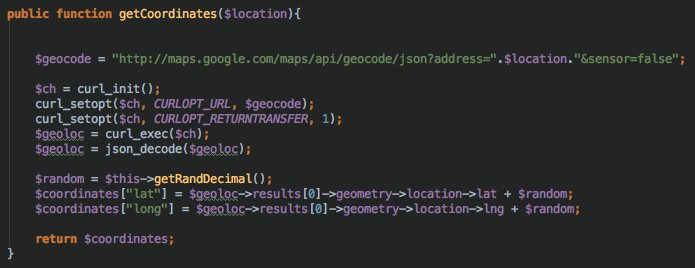
\includegraphics[width=1.0\textwidth]{imagenes/getGeocode.png}
\caption{Función que Obtiene los datos de Geolocalización de una ciudad}
\label{getCordinates-app}
\end{center}
\end{figure}

En esta capa se accede a los datos para ser modificados mediante los modelos datos y utilizando una herramienta de Laravel como ORM, facilita la conexión
con la base de datos. Estos métodos de ORM sustituyen a sentencias SQL. Por ejemplo: la función get() de una clase que extiende de la clase Model de Laravel
obtendría todos los registros de la tabla que se corresponde con ese modelo. En SQL el equivalente sería hacer un SELECT * FROM Tabla.


En los modelos además de conectarse con la base de datos, también hay métodos que conectan con API externas para recoger datos. Es el caso del método getCoordinates()
(figura \ref{getCordinates-app}) donde se llama a la API de Google Maps enviando un string con la localización de una ciudad y obteniendo sus datos de
geolocalización.


\textbf{Controladores}

En esta capa se encuentra la mayor parte de la lógica de la aplicación.Como se comentó previamente, existen varios controladores según para que
apartados de la web. Pero todas las rutas pasan por el controlador principal que las maneja y controla que existan para mostrar la vista correspondiente.

\begin{figure}
\begin{center}
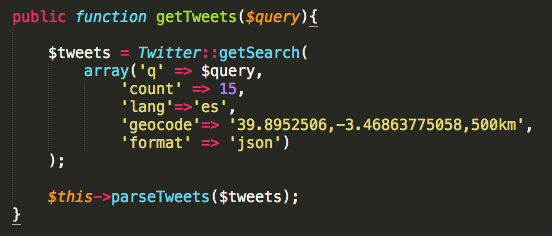
\includegraphics[width=1.0\textwidth]{imagenes/getTweets.png}
\caption{Función que recibe los datos de Twitter}
\label{getTweets-app}
\end{center}
\end{figure}

\begin{figure}
\begin{center}
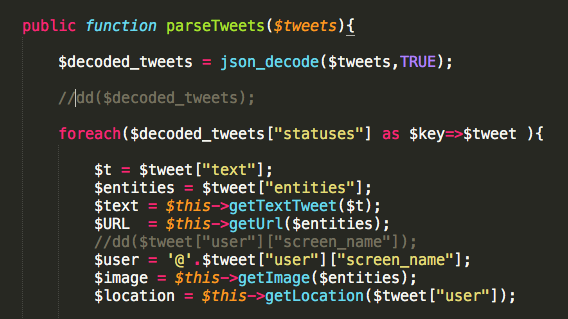
\includegraphics[width=1.0\textwidth]{imagenes/parseTweets.png}
\caption{Función para parsear los Tweets}
\label{parseTweets-app}
\end{center}
\end{figure}

\begin{figure}
\begin{center}
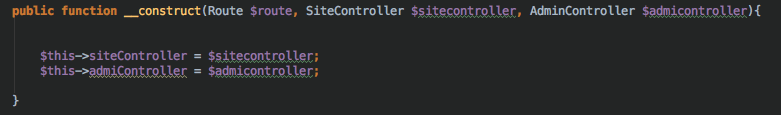
\includegraphics[width=1.0\textwidth]{imagenes/controller-constructor.png}
\caption{Constructor del controlador principal}
\label{controller-construct}
\end{center}
\end{figure}

\begin{figure}
\begin{center}
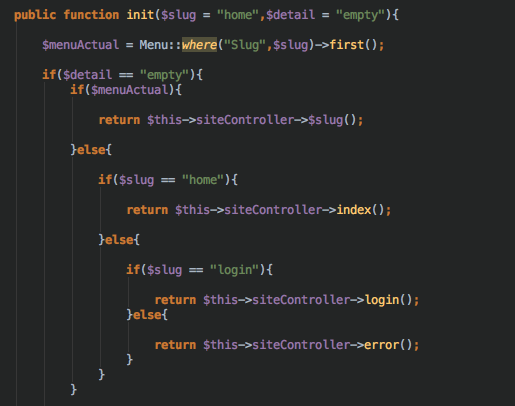
\includegraphics[width=1.0\textwidth]{imagenes/controller-init.png}
\caption{Método de init()}
\label{controller-init}
\end{center}
\end{figure}


\begin{figure}
\begin{center}
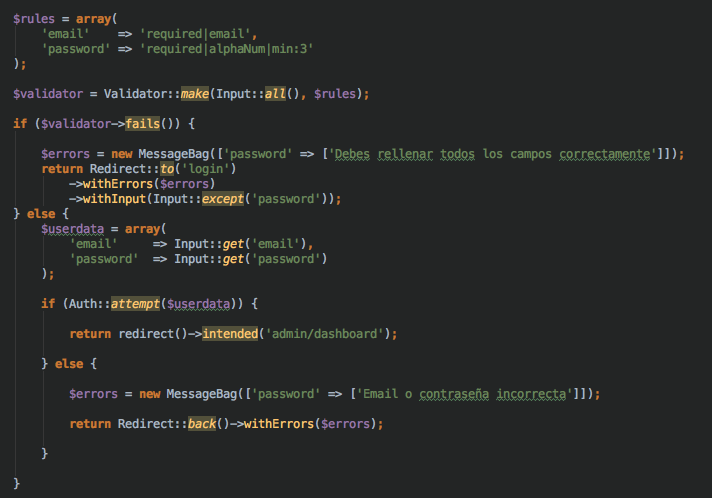
\includegraphics[width=1.0\textwidth]{imagenes/controller-login.png}
\caption{Método de login()}
\label{controller-login}
\end{center}
\end{figure}

\begin{figure}
\begin{center}
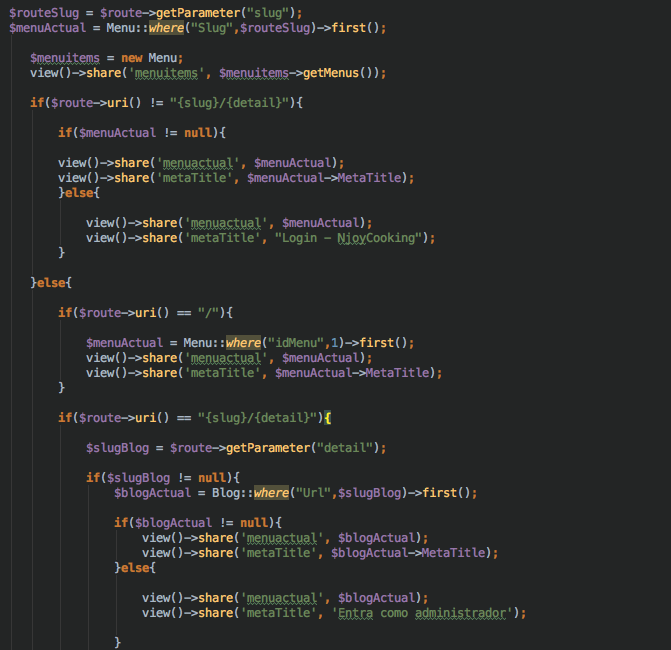
\includegraphics[width=1.0\textwidth]{imagenes/site-construct.png}
\caption{Constructor del siteController}
\label{site-construct}
\end{center}
\end{figure}

\begin{figure}
\begin{center}
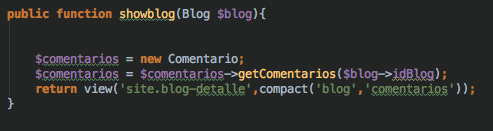
\includegraphics[width=1.0\textwidth]{imagenes/site-showblog.png}
\caption{Método shoBlog del siteController}
\label{site-showblog}
\end{center}
\end{figure}

Como se observa en \ref{controller-construct}, al inicializar el controlador, se generan dos instancias de los otros dos controladores que se encargan de manejar los datos y renderizar las vistas para la parte pública y la parte de administrador.

\vspace{5 mm}

Existen dos métodos dentro de la clase que controlan las rutas, init() para la parte pública e iniDashboard() para la parte que requiere loguearse.

\vspace{5 mm}

En el caso de la parte pública, en \ref{controller-init} se observa el método init(). Incialmente se le pasan los campos \$slug y \$detail que son los trozos de la url.
Se comprueba que el \$slug se encuentre en la tabla de menú de la base de datos y se empieza a buscar la url para mostrar la vista correspondiente. Por defecto si a los trozos de url que se pasan estan vacíos se establecen valores predeterminados. En el caso del \$slug cuando esta vacío es que es la url de inicio y por tanto se debe imprimir la página incial de la web. Para el caso \$detail si la url esta vacía se establce a empty, de esta forma sabemos que no se ha pasado ninguna url de detalle y por tanto se renderizan las páginas que no tienen detalle, como por ejemplo la página del mapa. Si la url contiene un detalle entonces pertenece a cada noticia del blog

\vspace{5 mm}

El login de la aplicación se gestiona también mediante el controlador principal. En el método doLoging() se realiza la identificación del usuario en la
aplicación. Como se observa en \ref{controller-login} inicialmente se validan los datos que el usuario ha introducido. En el caso de que la validación falle, devuelve al usuario a la página de login con los errores pertinentes. Si las credenciales del usuario son correctas se le redirige a la ruta de inicio del administrador.

\vspace{5 mm}

Las instancias de del siteController y el adminController que se usan en el controller, llaman a las diferentes funciones que gestionan los datos a
mostrar para cada vista. Antes de llamar a cualquier función se inicializa la clase mediante el constructor. Un ejemplo del constructor sería \ref{site-construct} donde se observa el código al inicalizar el siteController. En el constructor obtenemos el valor de la url en la que estamos y se obtienen los metas de la página  para introducirlos en el Html. También se guardan los datos de la página.

\vspace{5 mm}

Con la clase inicializada, se pueden llamar a las distintas funciones disponibles. Un ejemplo podría ser el método showBlog() del siteController,
 que muestra el detalle de cada noticia del blog. Como se observa en la figura \ref{site-showblog} se pasa por parámetro una variable blog que contiene
 el blog al que hemos accedido. Se recogen los comentarios relacionados a la noticia llamando al modelo correspondiente de los comentarios. Y por último
 se devuelve la vista correspondiente con la información asociada, en este caso los datos del blog y los comentarios.

 El caso más complejo de lógica es el del mapa de geoposicionamiento de recetas. Para obtener la información de Twitter se utiliza la una API rest
 para Laravel que proporciona varias funciones de búsqueda de información. Una vez integrada la API con el proyecto toda la información se procesa en el
 modelo Tweet. El método básico de este modelo es getTweets(\$query)(figura \ref{getTweets-app}) ya que en este método es donde se hace uso de la API
 de Twitter para obtener los resultados de la red social. Para realizar la búsquedase utiliza el método getSearch() de la API a la que se le pasa un
 array con los parámetros de búsqueda:


 \begin{itemize}

 \item \textbf{q}: la consulta o palabra clave sobre el que la api va a buscar los tweets. Es parámetro es dinámico ya que se pasa por parámetro en la función para que el administrador pueda modificar la palabra clave desde el dashboard.

 \item \textbf{count}: número de resultados que devolverá la consulta.

 \item \textbf{lang}: idioma en el que están los tweets.

 \item \textbf{geocode}: geocodificador que se le pasa por parámetro la latitud, longitud y un radio que representan el área sobre el que se van a buscar los tweets. El area utilizado es el de la península ibérica.

 \item \textbf{format}: el formato en el que devuelve los resultados. En este caso json.

 \end{itemize}


 Al resolver la petición, devuelve los tweets con toda la información asociada. Como no se van a utilizar todos los datos obtenidos esta información
 se procesa con el método parseTweets()(figura \ref{parseTweets-app}). En este método se recorren uno a uno cada tweet y se obtienen los datos relevantes
 para insertar en la base de datos utilizando otros métodos de la clase.
